\pagebreak 
\section*{}

In this section, we will first describe the methodology used to preprocess data from various sources to engineer the necessary features for the predictive model. Second, we will outline the model selection and evaluation process, and finally, we will discuss the methodology used to interpret the model predictions using SHAP techniques. For ease of reference, the data preprocessing and feature engineering pipeline is summarised in Figure \ref{fig:preprocessing}, and an overview of the model training and prediction interpretation methodology can be found in Figure \ref{fig:methodology}.

\begin{figure}[h]
    \centering
    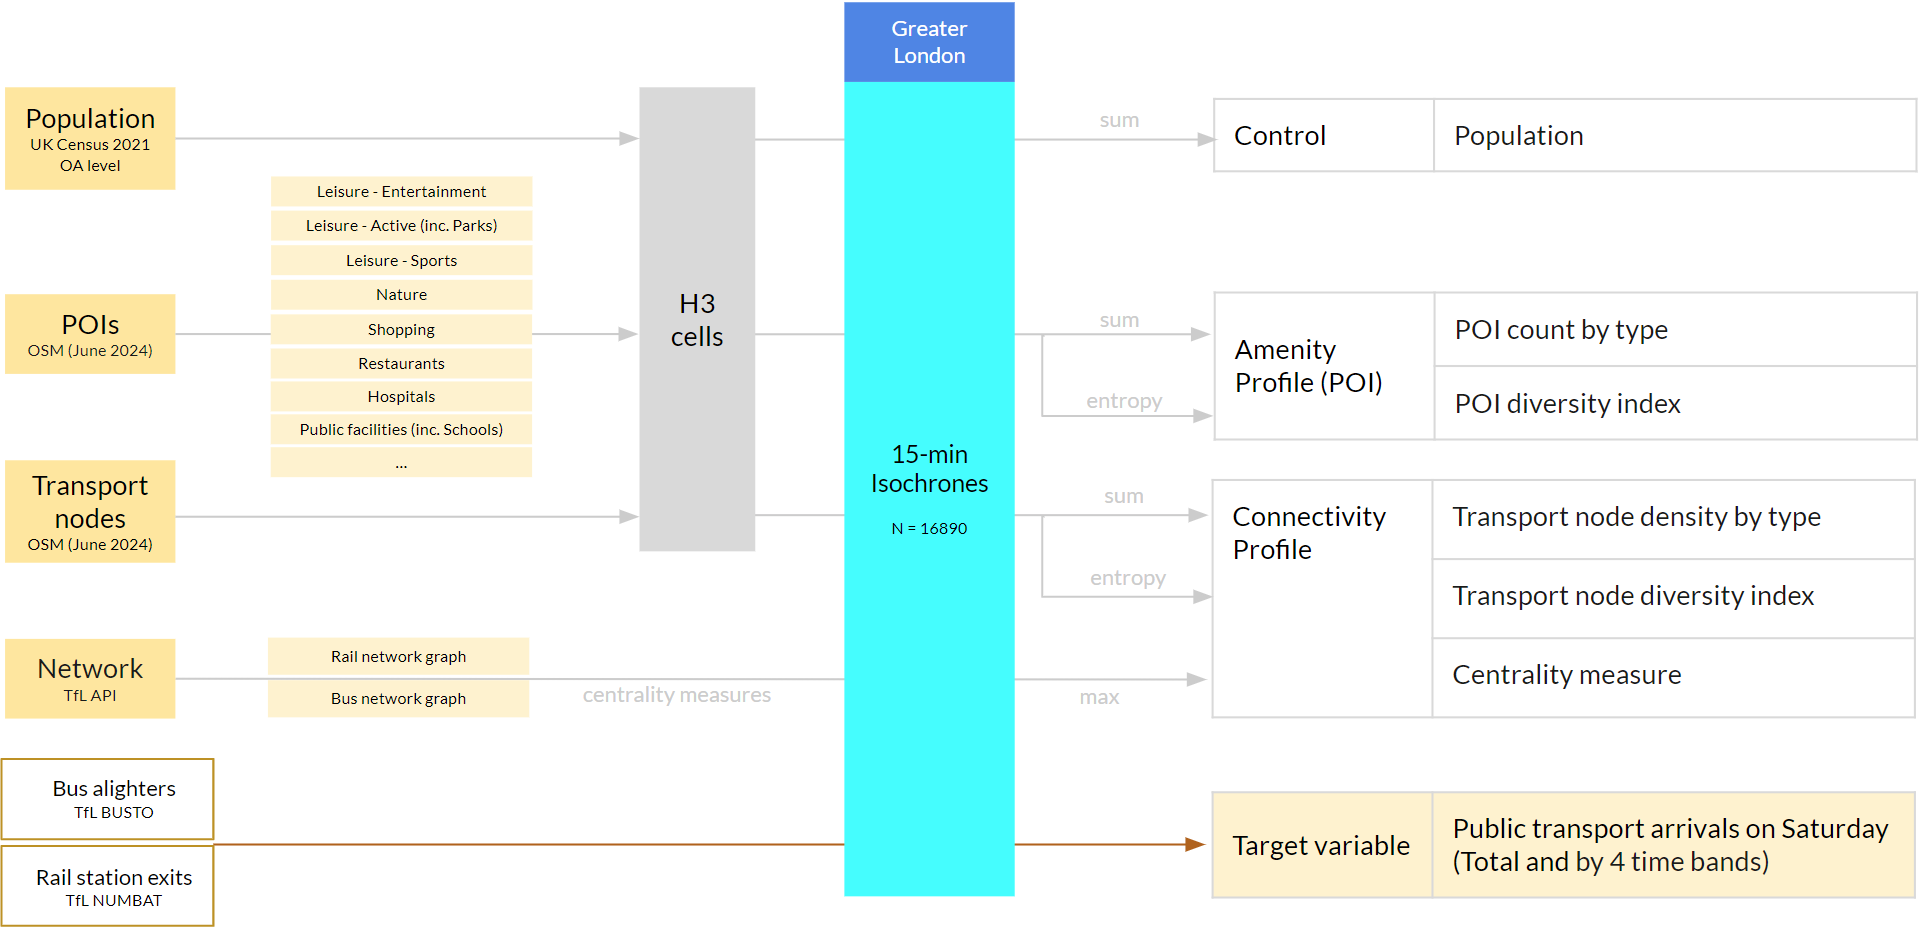
\includegraphics[width=\textwidth]{preprocessing.png}
    \caption{Overview of feature engineering pipeline}
    \label{fig:preprocessing}
\end{figure}

\begin{figure}[!ht]
    \centering
    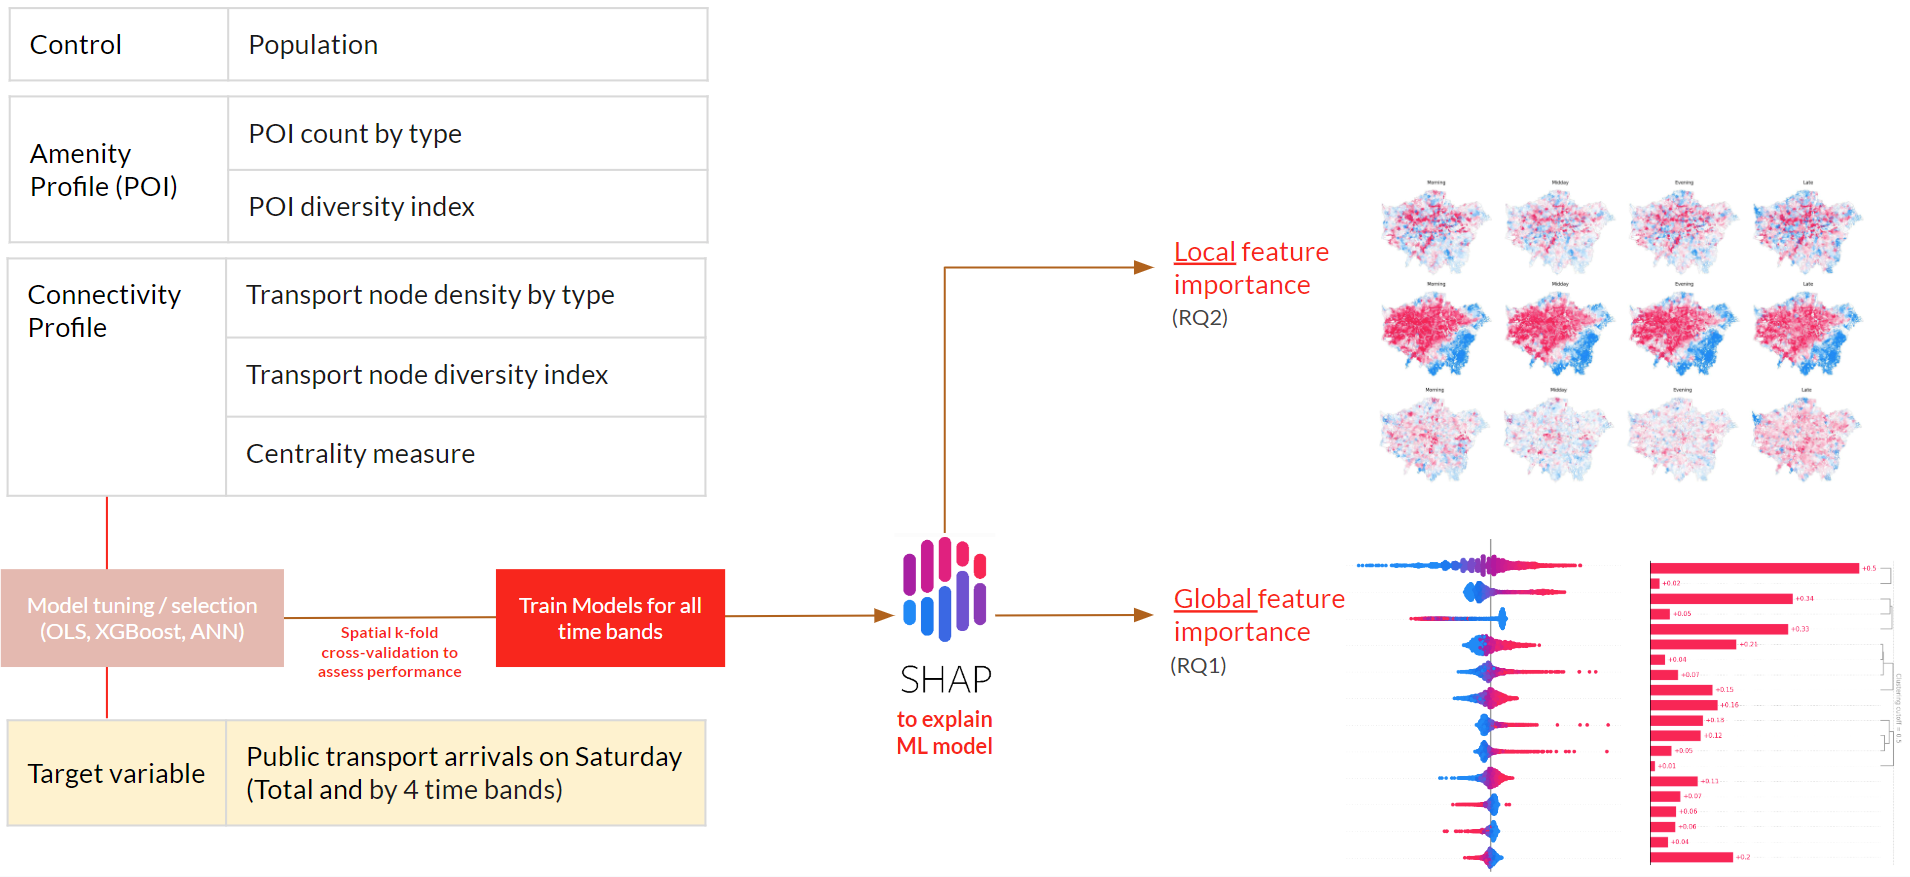
\includegraphics[width=\textwidth]{methodology.png}
    \caption{Overview of model training and interpretation}
    \label{fig:methodology}
\end{figure}

\pagebreak % Force a page break
\section{Open data sources}

The analysis carried out in this dissertation will utilise the Greater London area as the working case study, serving as an example for further replications of the analysis for other localities. The Office for National Statistics (ONS) defines the Greater London metropolitan area to include the City of London and the 32 London boroughs, with a total area of 1,572 km$^2$ and a population of 9.4 million people, making it the largest in the United Kingdom. The choice of the Greater London metropolitan area is also motivated by the availability of open data sources from which necessary features could be derived and the complexity of the public transport network that is coupled with rich usage data made available to the public. The data sources used in this analysis are summarised in Table \ref{tab:datasources} and detailed below.


\begin{table}[ht]
    \centering
    \renewcommand{\arraystretch}{1.5}
    \begin{tabular}{|l|l|l|}
        \hline 
        \rowcolor{lightgray}
        \textbf{} & \textbf{Variables} & \textbf{Sources} \\
        \hline

        \multirow{2}{12em}{\textbf{Public transport arrivals (target)}} 
        & Tube and Rail station exits & TfL network demand (NUMBAT) \\ 
        & Bus alightings & TfL network demand (BUSTO) \\
        \hline

        \textbf{Population} & Population count & UK Census 2021 \\
        \hline

        \multirow{2}{12em}{\textbf{Amenity Profile}} 
        & POI count by type & OSM Amenity POIs \\ 
        & POI diversity index & \\ 
        \hline 

        \multirow{3}{12em}{\textbf{Public Transport (PT) Connectivity Profile}} 
        & PT node count by type &  \\
        & PT node diversity index & OSM Transport POIs and TfL \\
        & PT network centrality &  \\
        \hline

            \end{tabular}
    \caption{Summary of data used in the analysis and their sources}
    \label{tab:datasources}
\end{table}

\subsubsection*{Transport for London (TfL) Open Data}

We use the following GIS datasets from the \href{https://gis-tfl.opendata.arcgis.com/}{TfL GIS Open Data Hub} and \href{https://api.tfl.gov.uk/}{TfL API} to derive transport-related features for the study area including density of transport facilities, diversity of transport options, and accessibility in the form of centrality measures in the Rail and Bus networks separately. The networks of interest are defined as follows:

\begin{itemize}
    \setlength\itemsep{0em}
    \item \textit{Rail network} includes the London Underground, London Overground, the Docklands Light Railway, and the Elizabeth Line, excluding stations and segments that are not managed by TfL or fall outside the Greater London area.
    \item \textit{Bus network} includes stop locations and route data of all bus and tram services, excluding stops and route segments that are not managed by TfL or within the Greater London area.
\end{itemize}

TfL also provides annually-updated \href{http://crowding.data.tfl.gov.uk/}{network demand datasets}, which will be used to derive the target variable of our analysis. The datasets are special interest to our analysis are namely \textit{Rail demand data (NUMBAT)} and the \textit{Bus demand data (BUSTO)}, from which we will extract estimated counts of station exits and bus alightings at the station or stop level, respectively. The dataset's temporal granularity is also an important aspect to consider. To address non-commute trips for the analysis, we will specifically use \textbf{Saturday average demand}, representing the demand in a typical period without any major citywide disruptions or events\footnote{This Saturday travel demand may still include work trips for those working on Saturdays, albeit not concentrated into peak periods as with weekday travel demand. For the scope of this analysis, we will treat these potential work trips as non-commute.}. To examine possible variations between different times of day, besides the total daily counts of exits and bus alightings, we will aggregate the data into four larger time bands\footnote{The choice of time band delineation is a compromise between different granularity levels afforded by the TfL rail and the bus demand datasets. There are opportunities to deepen the analysis by further segmenting the time bands into finer intervals, if data permits.}:

\begin{itemize}
    \setlength\itemsep{-0.2em}
    \item \textit{Morning} (05:00 - 10:00): Limited mobility expected due to early hours
    \item \textit{Midday} (10:00 - 19:00): High daytime mobility expected
    \item \textit{Evening} (19:00 - 00:00): High evening mobility expected
    \item \textit{Late} (00:00 - 05:00): Minimal mobility expected due to sparser night PT services
\end{itemize}

It is worth noting that despite the existence of the Oyster Card integrated fare system, TfL does not provide origin-destination data for individuals as open data. Therefore, station exits and bus alightings are not directly associated with the number of passengers traversing through the system but are treated as discrete events. For example, a person who takes a bus to reach a Tube station for onward travel and then exits to arrive at their destination would be counted as two separate data points, one alighting for the bus and one station exit for the Tube. Nevertheless, our model will take this into account when making porediction and allows us to investigate patterns and the contribution of modal interchange behaviour in our interpretation.

Lastly, we need to acknowledge the particularity of the TfL bus demand dataset (BUSTO). Although passengers do not 'tap off' when alighting from busses, TfL has developed a methodology to estimate the number of passengers alighting at each bus stop based on individuals' next actions and other statistical methods. The methodology is described in detail in the \href{http://crowding.data.tfl.gov.uk/BUSTO/BUSTO\%20User\%20Guide\%20and\%20Data\%20Dictionary\%20v1.0.pdf}{BUSTO User Guide and Data Dictionary}

\subsubsection*{UK Census Data 2021}
For the estimated population datasets, we rely on the most recent United Kingdom Census data administered in 2021. The data is ingested at the Output Area (OA) level, which is the smallest geographical unit for which census data is available. Further processing will aggregate the data to the desired spatial unit of analysis.

\subsubsection*{OpenStreetMap POIs}
OpenStreetMap (OSM) is a collaborative mapping project that provides a free and open-source map of the world. The version of OSM data used in this analysis is packaged by an OpenStreetMap community project \href{https://www.geofabrik.de/en/geofabrik/openstreetmap.html}{Geofabrik} and provides a snapshot of the OSM database as of June 2024. Geofabrik also standardises the categorisation of POIs' amenity attributes in the OSM database into larger classes\footnote{More information about Geofabrik's OSM data product can be found in \href{https://www.geofabrik.de/data/geofabrik-osm-gis-standard-0.6.pdf}{Geofabrik OSM data dictionary}}. Our analysis will use this default POI classification, extracting 12 amenity POI types. Lastly, apart from amenity POIs, we also make use of the OSM transport POIs point data to derive non-TfL transport-related features, such as national rail stations, ferry piers, long-distance bus stations and airports. 

Combined with transport node data acquired from TfL open data sources, all extracted Amenity and Transport POI types of interest are summarised in Table \ref{tab:osmpoi}.

\begin{table}[ht]
    \centering
    \renewcommand{\arraystretch}{1.1}
    \begin{tabular}{|l|l|l|}
        \hline
        \rowcolor{lightgray}
        & \textbf{POI Type} & \textbf{Examples} \\
        \hline
        \multirow{13}{*}{\textbf{Amenity}}
            &\textit{Public Facilities} & Post offices, schools, universities, libraries,... \\
            &\textit{Medical} & Hospitals, clinics, pharmacies,... \\
            &\textit{Entertainment} & Theatres, Night clubs, cinemas,... \\
            &\textit{Outdoors} & Parks, playgrounds,... \\
            &\textit{Active} & Sports centres, swimming pools, stadiums,... \\
            &\textit{Restaurants} & Restaurants, cafes, pubs, bars,... \\
            &\textit{Hotels} & Hotels, motels, hostels,... \\
            &\textit{Shopping} & Supermarkets, bakeries, florists, bookshops, malls,... \\
            &\textit{Banking} & Banks, ATMs,... \\
            &\textit{Tourism} & Tourist attractions, museums, monuments, viewpoints,... \\
            &\textit{Religious} & Churches, mosques, temples,... \\
            &\textit{Nature} & Riverbanks, beaches, hills,... \\
        \hline
        \multirow{3}{*}{\textbf{Transport}}
            &\textit{Bus stops} & Bus stops and stations (TfL) \\
            &\textit{Rail stations} & TfL rail stations (TfL) and Non-TfL rail stations (OSM) \\
            &\textit{Other transport hubs} & Airports, ferry piers, long-distance bus stations (OSM) \\
        \hline
    \end{tabular}
    \caption{Summary of Amenity and Transport POI types used in the analysis}
    \label{tab:osmpoi}
\end{table}


\pagebreak % Force a page break
\section{Defining the spatial unit of analysis}

As features will be extracted and engineered from different data sources, the spatial unit is an important consideration, at which the features are aggregated, and the Machine Learning model is trained. In this analysis, we will use 15-minute walking isochrones---i.e., the area that can be reached within a 15-minute walk from a given point---as the spatial unit of analysis. The isochrones were generated based on initial seeds of 16,890 points across the Greater London area, using the pedestrian profile of the OpenStreetMap Network API (osmnx), which takes into account pedestrian infrastructure such as footpaths, pedestrian crossings, and pedestrianised areas. The choice of using isochrones as the spatial unit of analysis for our model is motivated by the following reasons: 

\begin{itemize}
    \setlength\itemsep{0em}
    \item First, the spatial unit of aggregation and analysis for the model must reflect how individuals interact with transport nodes and amenity POIs that are accessible using the existing pedestrian network. Proximity using the Euclidean distance is inaccurate when there are natural barriers such as rivers, or private estates that prevent through access. 
    \item Second, human mobility in cities is not bound by administrative boundaries such as Output Areas or boroughs, and the use of overlapping isochrones allows us to capture the spatial heterogeneity of the urban environment in our dataset.
    \item Third, the 15-minute specification of the isochrones aims to reflect a uniformity among the spatial units of analysis while following a predetermined standard set out by the 15-minute city concept that characterises the extent of desirable mobility in a neighbourhood.
    \item Lastly, the density of the isochrones produced is a compromise between the granularity of the spatial unit and the computational resources required to process the data. The initial seeds of 16,890 points are originally centroids of the same number of H3 cells at resolution 9 needed to cover the Greater London area. 
\end{itemize}

The detailed methodology to generate the isochrones is illustrated in Figure \ref{fig:isochrones}, and two example isochrones in Central London can be found in Figure \ref{fig:isozoom}. It is worth noting that depending on where the spatial unit is located in the Greater London area, the isochrones may vary in shape and size due to the underlying pedestrian network and the distribution of transport nodes and amenity POIs. However, these variances are expected and even desirable as they more closely reflect pedestrian accessibility to different types of amenities and transport nodes. All raw data extracted from various sources will be aggregated and processed at the isochrone level to generate the necessary features and target variable for the model training (See Figure \ref{fig:preprocessing}). In the next section, we will describe the data transformation and feature engineering process in more detail. Note that the terms spatial units (of analysis), isochrones, or simply areas may be used interchangeable from this point on in our discussion.

\begin{figure}[ht]
    \centering
    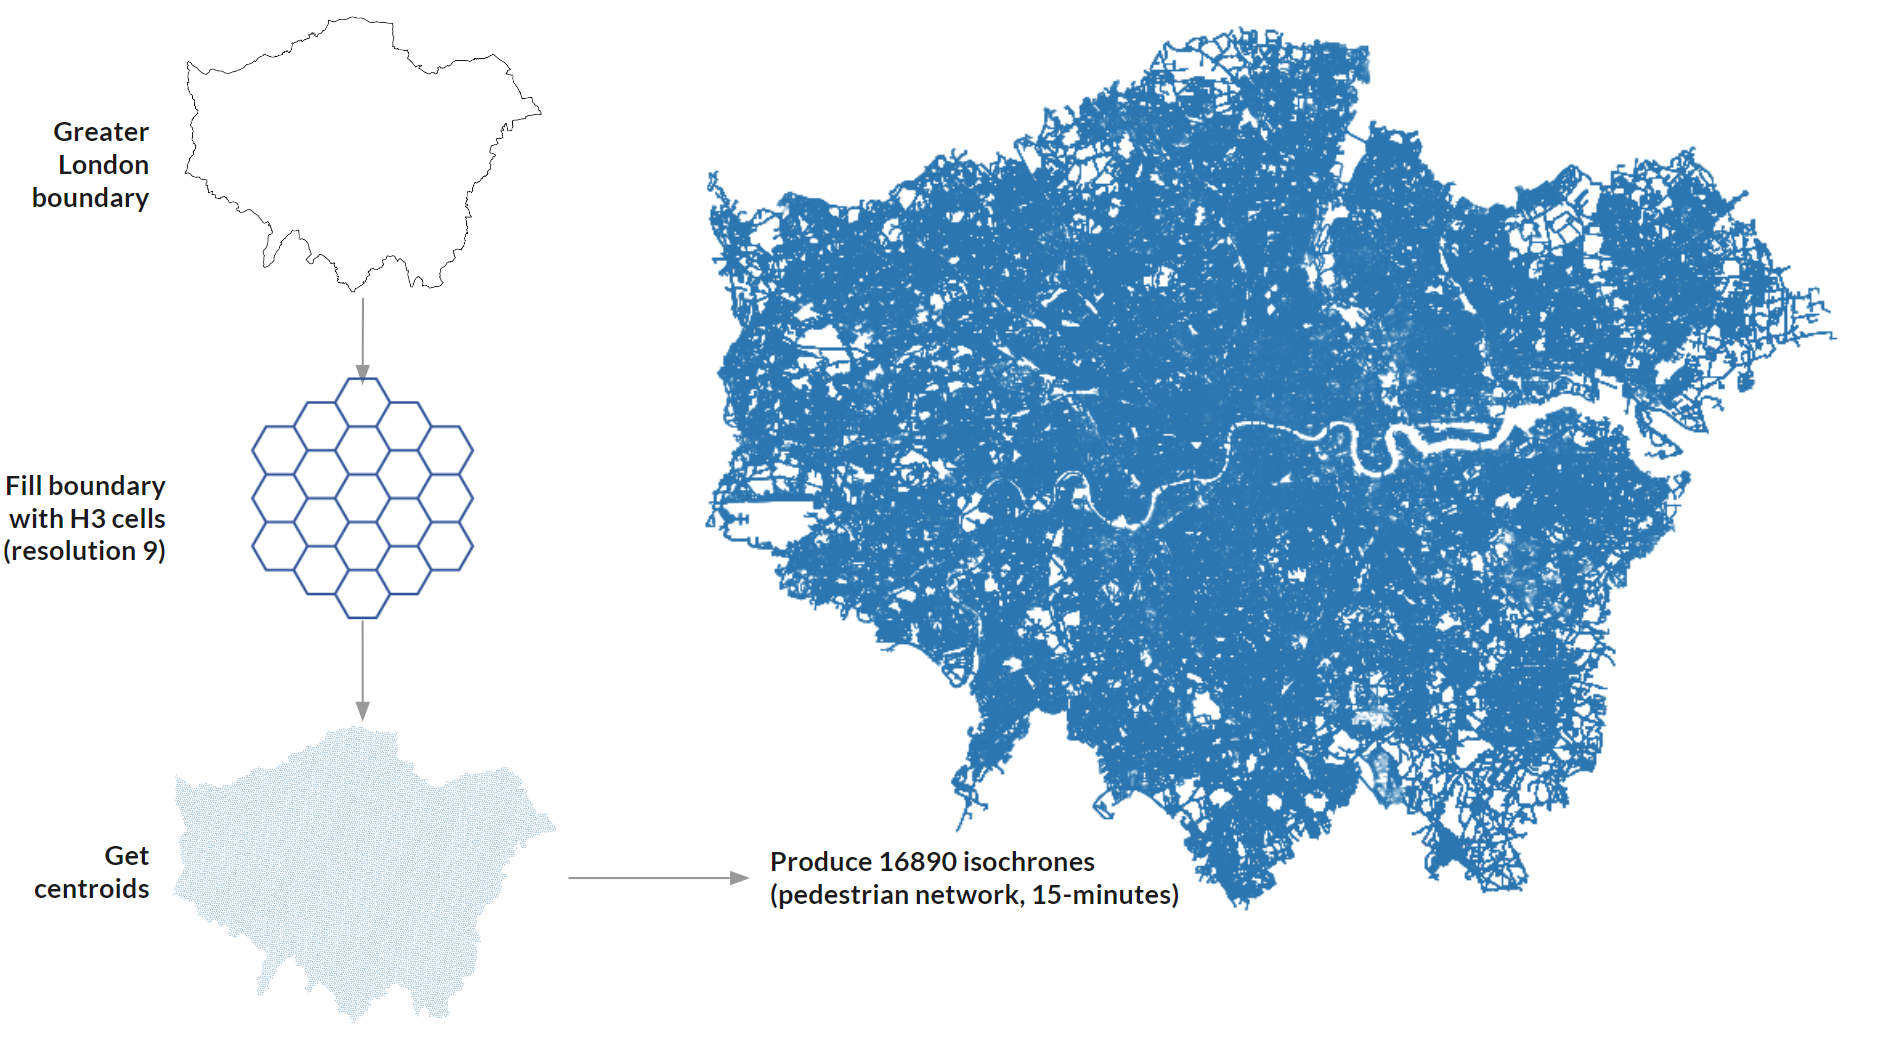
\includegraphics[width=0.8\textwidth]{isochrones.png}
    \captionsetup{justification=centering}
    \caption{Methodology to generate 15-minute walking isochrones as the spatial unit of analysis}
    \label{fig:isochrones}
\end{figure}

\begin{figure}[!ht]
    \centering
    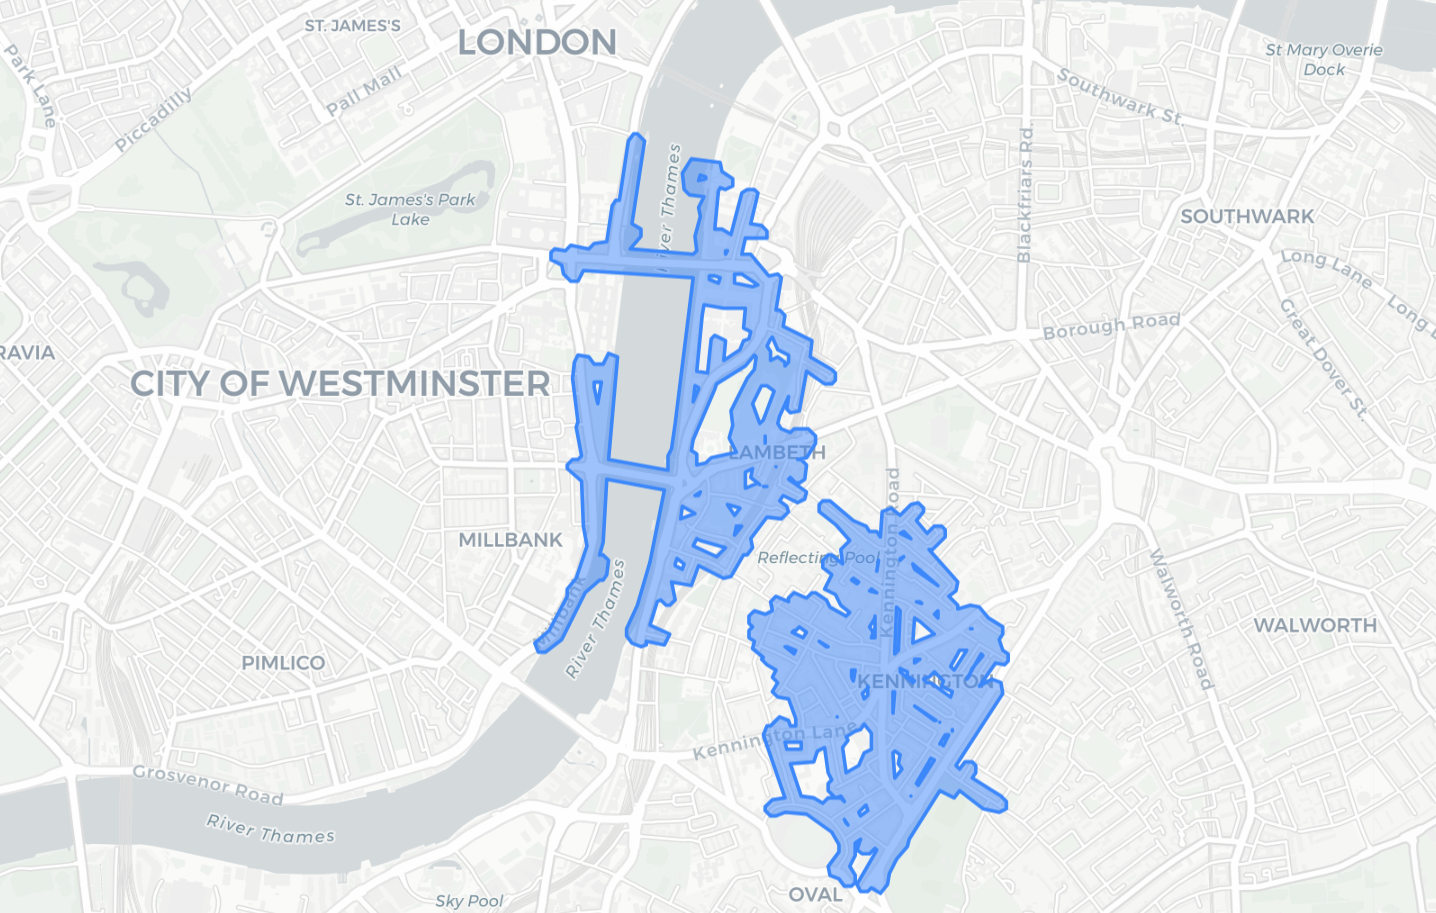
\includegraphics[width=0.7\textwidth]{isozoom.png}
    \caption{Two example spatial units of analysis located in Central London}
    \label{fig:isozoom}
\end{figure}




\pagebreak[4] % Force a page break
\section{Data Preprocessing}
\subsection{Aggregating target variables}


The total numbers of passengers who arrive at a transport node or alight from a bus at a stop are the target variables for our model, used to train the model to predict the number of passengers arriving at a transport node or alighting from a bus at a given isochrone. 
The aggregation results are illustrated in Figure \ref{fig:ptarrival}, which shows the total daily figures as well as the figures aggregated into the four time bands described earlier in order to capture the temporal variations. The total daily figures show a clear concentration of passenger arrivals in the Central London area, with the highest number of passengers arriving at transport nodes in the morning and evening time bands. The time band figures show a similar pattern, with the highest number of passengers arriving during the Midday time band (10:00-19:00). The Evening time band also shows a significant number of passengers arriving at transport nodes, while the Morning and Late time bands show lower numbers of passengers using the system, due to early hours in the day on weekends and sparser night services, respectively.

\begin{figure}[!b]
    \centering
    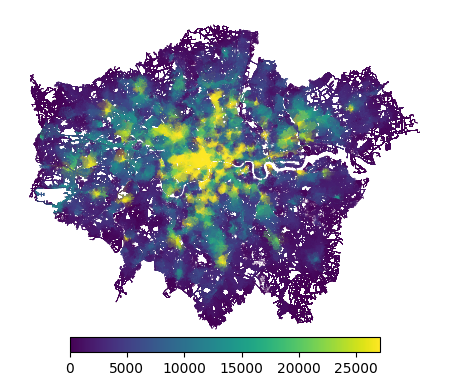
\includegraphics[width=0.6\textwidth]{pt_arrival_total.png}
    \centering
    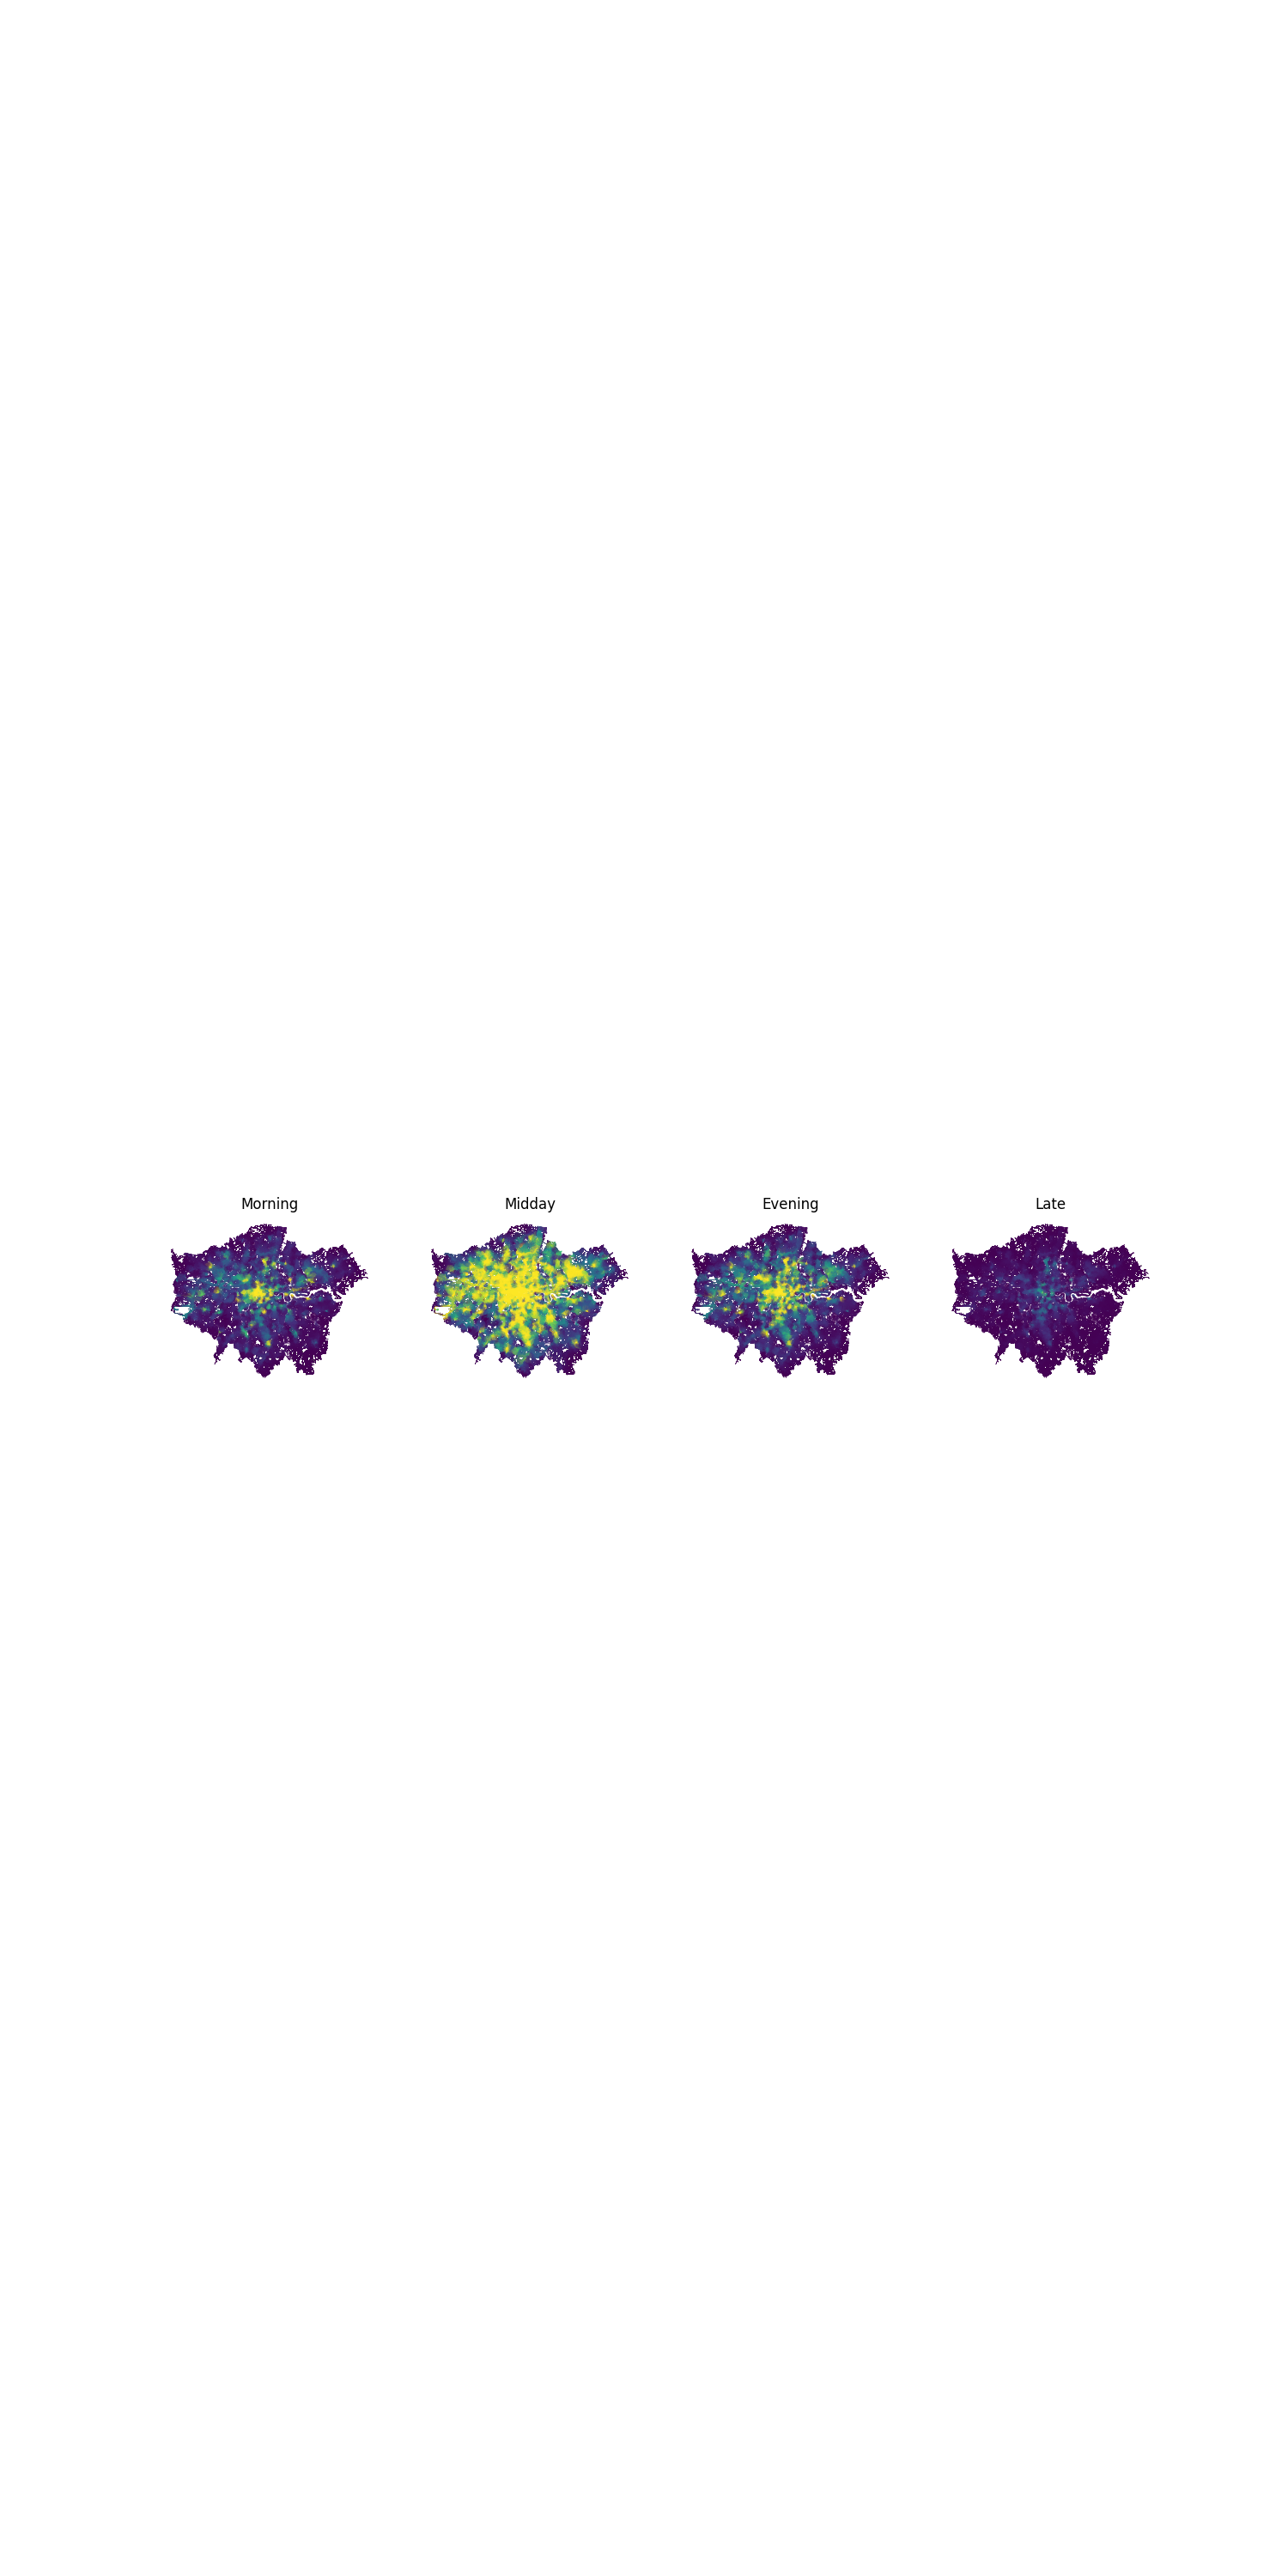
\includegraphics[width=\textwidth]{pt_arrival_timeband.png}
    \captionsetup{justification=centering}
    \caption{Aggregated arrivals at the chosen spatial unit level\\ by total daily (top) and by time band (bottom)}
    \label{fig:ptarrival}
\end{figure}

Lastly, since the target variable has a highly right-skewed distribution, we will apply a log transformation to the target variable to normalise the distribution and improve the model's performance. The log transformation of the target variable is shown in Figure \ref{fig:rawlog}, which shows a more normal distribution of the target variable after the transformation. The log-transformed target variable will be used in the model training and evaluation process, and will be implicit from this point on.

\begin{figure}[!ht]
    \centering
    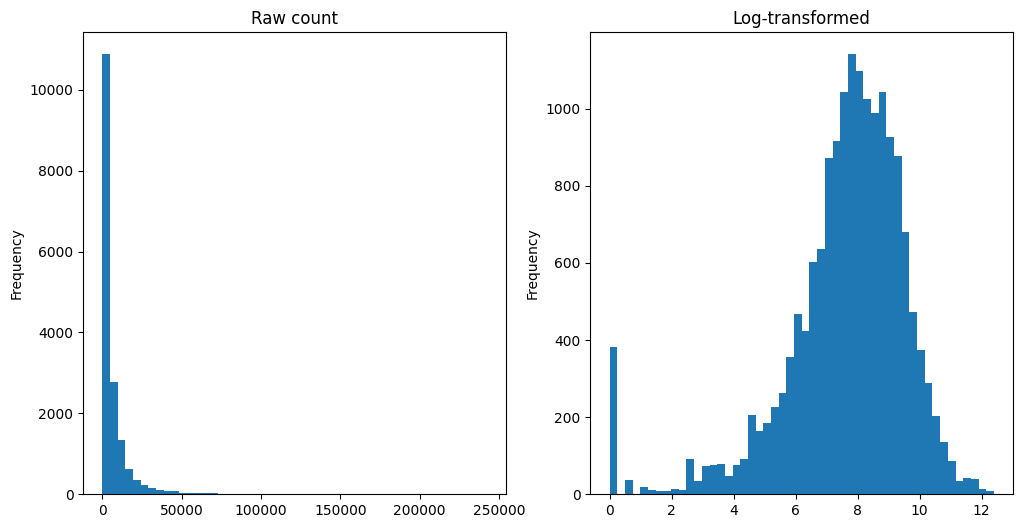
\includegraphics[width=0.65\textwidth]{raw-log.png}
    \captionsetup{justification=centering}
    \caption{Distribution of the Total arrivals as raw count (left) and log-transformed (right). Similar transformations carried out for arrivals by each of the four time bands}
    \label{fig:rawlog}
\end{figure}
\subsection{Feature engineering}
\subsubsection*{Density}

Density of POIs is one of the first feature type of interest for our model \citep{cerveroTravelDemand3Ds1997}, which represents the presence intensity of amenities or transport nodes of each type in an area that would attract visitors (in our case, coming by public transport). We expect a positive correlation between the density of POIs of all types to the total number of arrivals. An area with a high concetration of retail within a 15-minute walk is expected be more attractive than a similar-sized area with a low concetration of retail. Similarly, an area with a high concentration of transport facilities such as stations, bus stops are expected to be accommodating a higher inflow volume of visitors. However, feature importance and spatial nonstationarity (different impact on the target variable depending  the location) in this regard will be factors of interest as we interpret the model predictions post-training.

All density-related features---i.e., population, amenity POI density and transport node POI density---are formulated by aggregating their values for each spatial unit (isochrone) by type, resulting in a set of \textbf{16 features} (See Figure \ref{fig:poi} in the Appendix)

\subsubsection*{Diversity}

Diversity of Amenity POIs according to \citet{cerveroTravelDemand3Ds1997} is also an important factor that may influence attractiveness of an urban area for certain type of non-commute travel demand. The implication from their conclusion is that between two areas with all else being equal, the area that is more diverse in the types of amenities it provides will be more attractive on average, because of their vibrancy and the possibility it can affords visitors to accomplish different tasks in one trip.

- Transport POI diversity

\citet{cerveroTravelDemand3Ds1997} conceptualised diversity in the form of \textit{entropy}. A concept originated in information theory, entropy is the average amount of information conveyed by an event when considering all possible outcomes. \citet{battyEntropyComplexitySpatial2014} further adapted it to convey complexity in a spatial system. Interestingly, they also considered the increasing spatial entropy to mean a trade-off between density of amenity types and the unique types of amenity present, which stands in competition with other density-based features created. Therefore, the inclusion of entropy as a measure of POI diversity may improve the model prediction accuracy.

Although there are many formulation for the calculation of entropy, we intend to replicate the methodology used by both of the cited works above and adopt the formulation of entropy introduced by \citet{shannonMathematicalTheoryCommunication1948} as follows:

- formula

Mapping

- map

% Add plots of diversity index for 3 boroughs


\subsubsection*{Centrality}
- Which 3 centrality measures are used

% Add plots of network


% Add plots of centrality measures

- Why not multi-Layered network
\subsection{Incorporating spatial lags as feature}

When working with machine learning models with data exist in a closed spatial system such as the Greater London area, it is important to consider the spatial autocorrelation in the target variables. Spatial autocorrelation refers to the phenomenon where the value of a variable at one location is correlated with the value of the same variable at nearby locations. In the context of our analysis, this means that the number of passengers arriving at a transport node or alighting from a bus at one isochrone is likely to be correlated with the number of passengers arriving at nearby isochrones. Although deep learning models' parameters and hyperparameters can be made more complex and tuned to reach a high degree of prediction accuracy without considering the spatial aspect of the dataset and can practically be considered non-parametric (i.e., not assuming the variables to have a specific distributions), accounting for potential spatial autocorrelation could reduce probability of biased outcomes even with a low-complexity and high-interpretability atchitecture, e.g. tree-based \citep{meyerImportanceSpatialPredictor2019}.

The existence of spatial autocorrelation in the target variables is confirmed by the Local Indicators of Spatial Association (LISA) analysis, which shows the presence of spatial clusters in the target variables (Figure \ref{fig:lisacluster}), using Local Moran's I indicators. High-High and Low-Low clusters of the total daily arrivals with public transport are respectively present in the inner core and the outer edge. Unless spatial relational information among these spatial units are made apparent to the model during tuning and evaluation, we are bound to see low accuracy espeically in these localities that make up more than 50\% of the study area.  

\begin{figure}[ht]
    \centering
    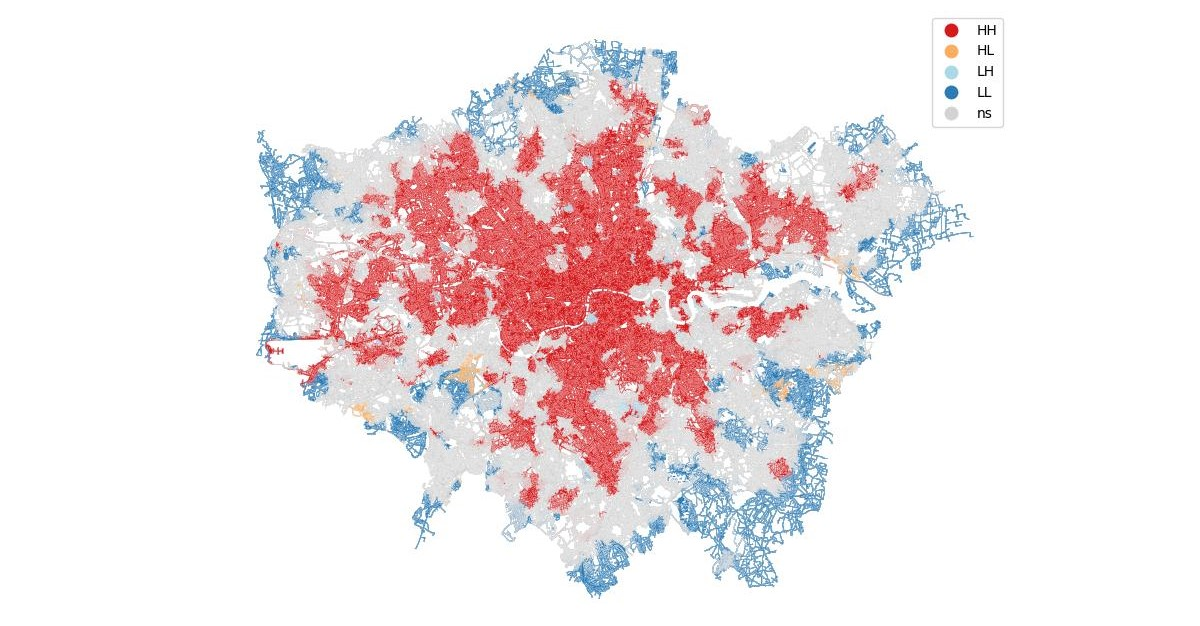
\includegraphics[width=\textwidth]{lisa_Total.jpg}
    \captionsetup{justification=centering}
    \caption{LISA cluster map of PT arrival volume (Total daily)\\Global Moran's I: 0.742 (High spatial autocorrelation)}
    \label{fig:lisacluster}
\end{figure}

To address this issue, \citet{liuIncorporatingSpatialAutocorrelation2022} has proposed incoporating spatial lag into the model as a feature. More specifically, the authors have concluded that when spatial features were induced in the random forest models, the global spatial autocorrelation among the predictions' residuals was significantly reduced, also leading to higher validation accuracy. For our analysis, the spatial lag feature of each spatial unit is calculated as the average number of passengers arriving at neighbouring isochrones\footnote{The choice of the distance band of 750m was calibrated with the objective to ensure all spatial units have neighbours, i.e., there are no islands.}. The creation of a \textbf{Spatial Lag features} is replicated for the total daily arrival counts, as well as for each time band, resulting in a set of additional features that will be included for the training of the model in predicting the corresponding target variable,

\begin{table}[ht]
    \centering
    \renewcommand{\arraystretch}{1.5}
    \begin{tabular}{|c r || r c l|}
        \hline
        \rowcolor{lightgray}
        \textbf{No.} & \textbf{Target variable} & \textbf{Main Features} & &\textbf{Spatial Lag Feature}\\
        
        \hline
        1 & Total arrivals  &  \multirow{5}{12em}{Population, amenity and transport profile features (25 features)} 
                                &  \multirow{5}{*}{+}       &   Lag - Total arrivals    \\ 
        2 & Morning arrivals    &                       &   &   Lag - Morning arrivals  \\ 
        3 & Midday arrivals     &                       &   &   Lag - Midday arrivals   \\ 
        4 & Evening arrivals    &                       &   &   Lag - Evening arrivals  \\ 
        5 & Late arrivals       &                       &   &   Lag - Late arrivals     \\
        \hline
    \end{tabular}
    \caption{Mapping spatial lag features to corresponding models to predict target variables}
    \label{tab:spatiallag}
\end{table}


\pagebreak % Force a page break
\section{Model selection and evaluation}
- Comparing Linear, XGBoost, ANN

- Preference for XGBoost, to be evaluated in Results
\section{Explainable machine learning with SHAP}
 - What is SHAP 
 
 - SHAP use cases for different machine learning models

 - SHAP for spatial

 - True to Data, True to Model

 - Limitations and comparisons to econometric models
